%!TEX root = ../../main.tex


\begin{figure}[!htb]
\centering
%\hrulefill \\
%\vspace{5pt}
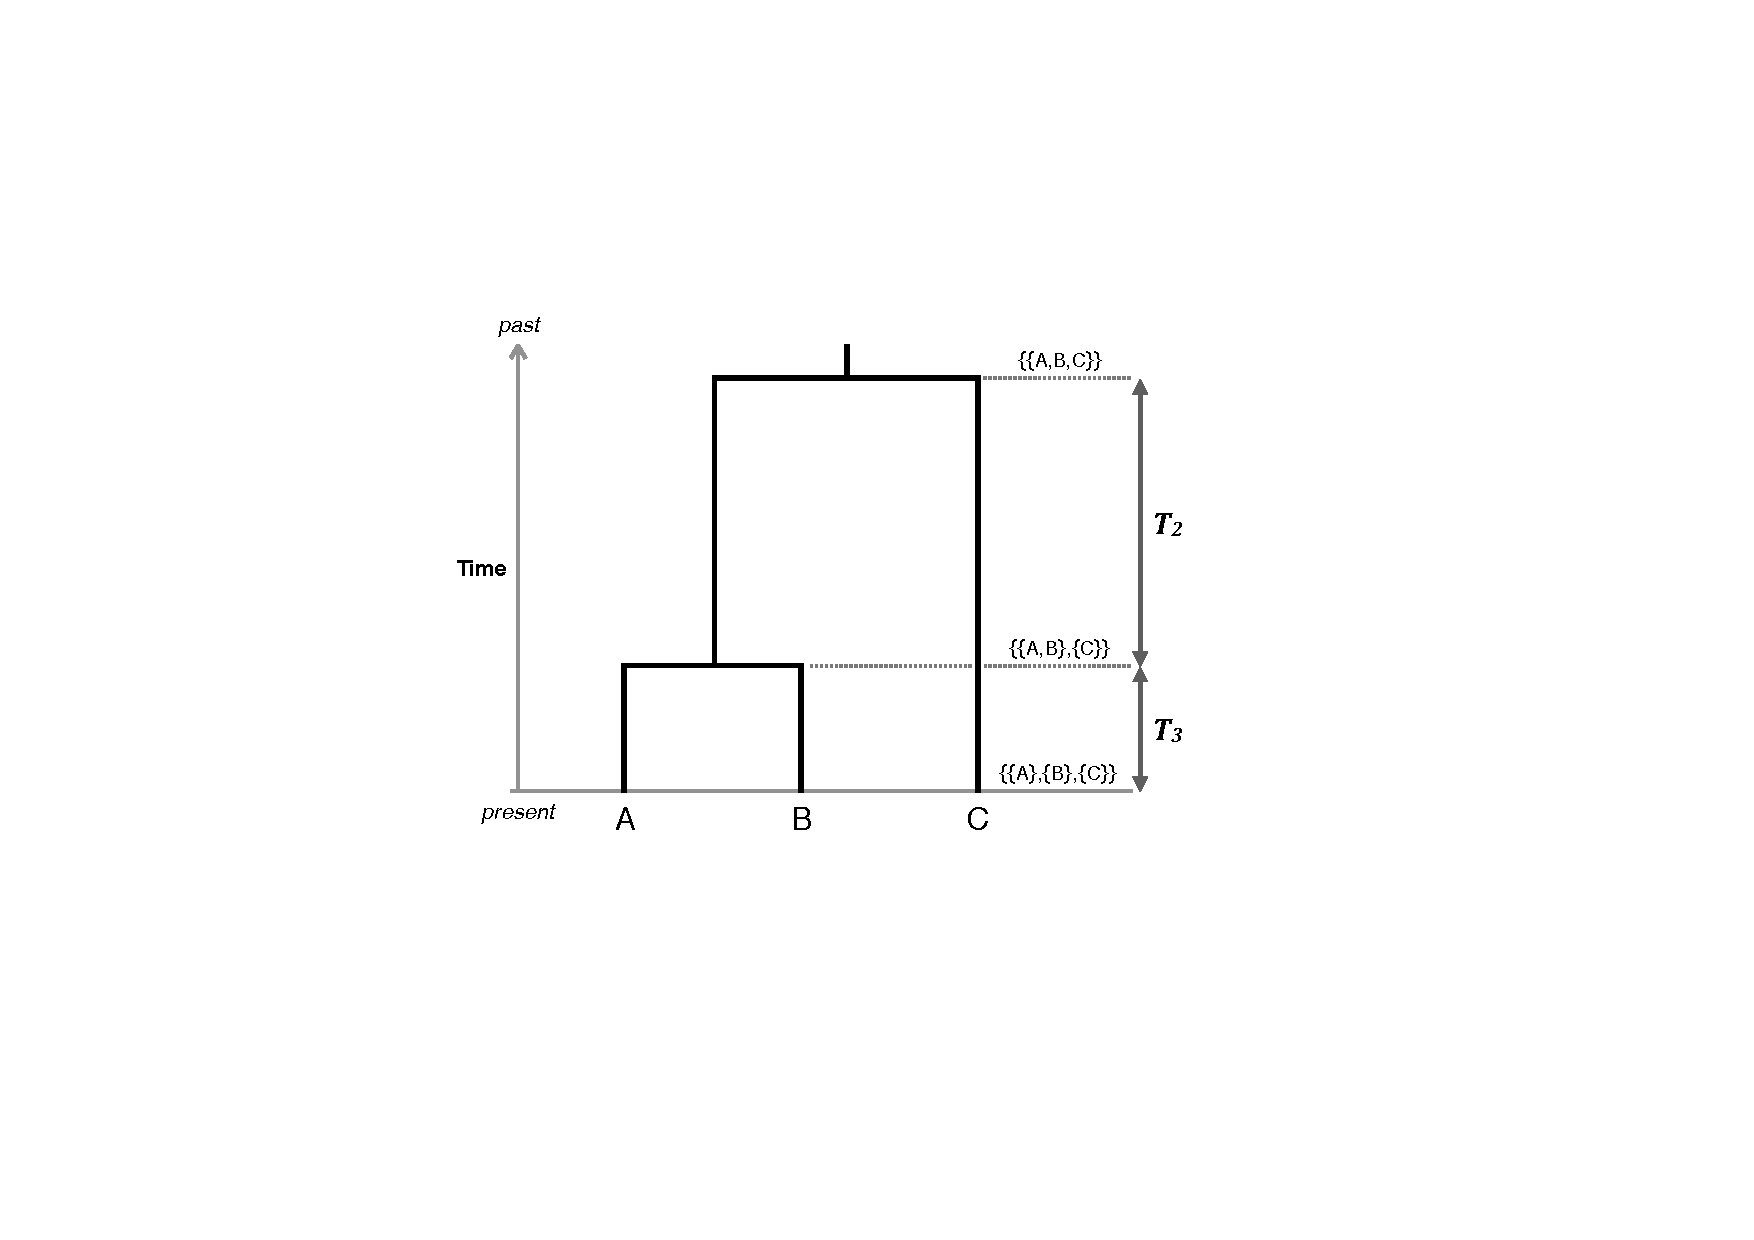
\includegraphics[width=0.7\textwidth]{./img/ch1/info_coalescent}
\Caption{Topology of a genealogical tree in the coalescent}
{The genealogical relationship of \n{3} haploid individuals is shown, $A$, $B$, and $C$, which represent separate lineages at present, but where $A$~and~$B$ are the first to coalesce (back in time).
The waiting time between successive coalescent events is denoted by \Correct{$T_i$}, where \Correct{$i$} is the number of ancestral lineages at a given time interval, which changes from \Correct{$i$} to \Correct{${i-1}$} at coalescence.
Figure modified from \citet{nordborg2001coalescent}.}
{fig:info_coalescent}
% \vspace{-5pt}
% \hrulefill%
\end{figure}
